%!TEX root = ../dissertation.tex
\chapter{Sviluppo}\label{ch:sviluppo}
In questa sezione, verranno introdotte le tecnologie che sono state utilizzate nel progetto di stage e verrà descritto come sono state integrate. 
\\
All'interno delle sezione di integrazione capiremo come è stato possibile costruire un sistema che si occupi di selezionare i file corretti da leggere, importare il contenuto manipolato all'interno di un applicativo interrogabile dall'esterno, avviare delle analisi sui dati e creare dei report sugli stessi.
\section{Integrazione}
\begin{figure}[h!]
	\centering
	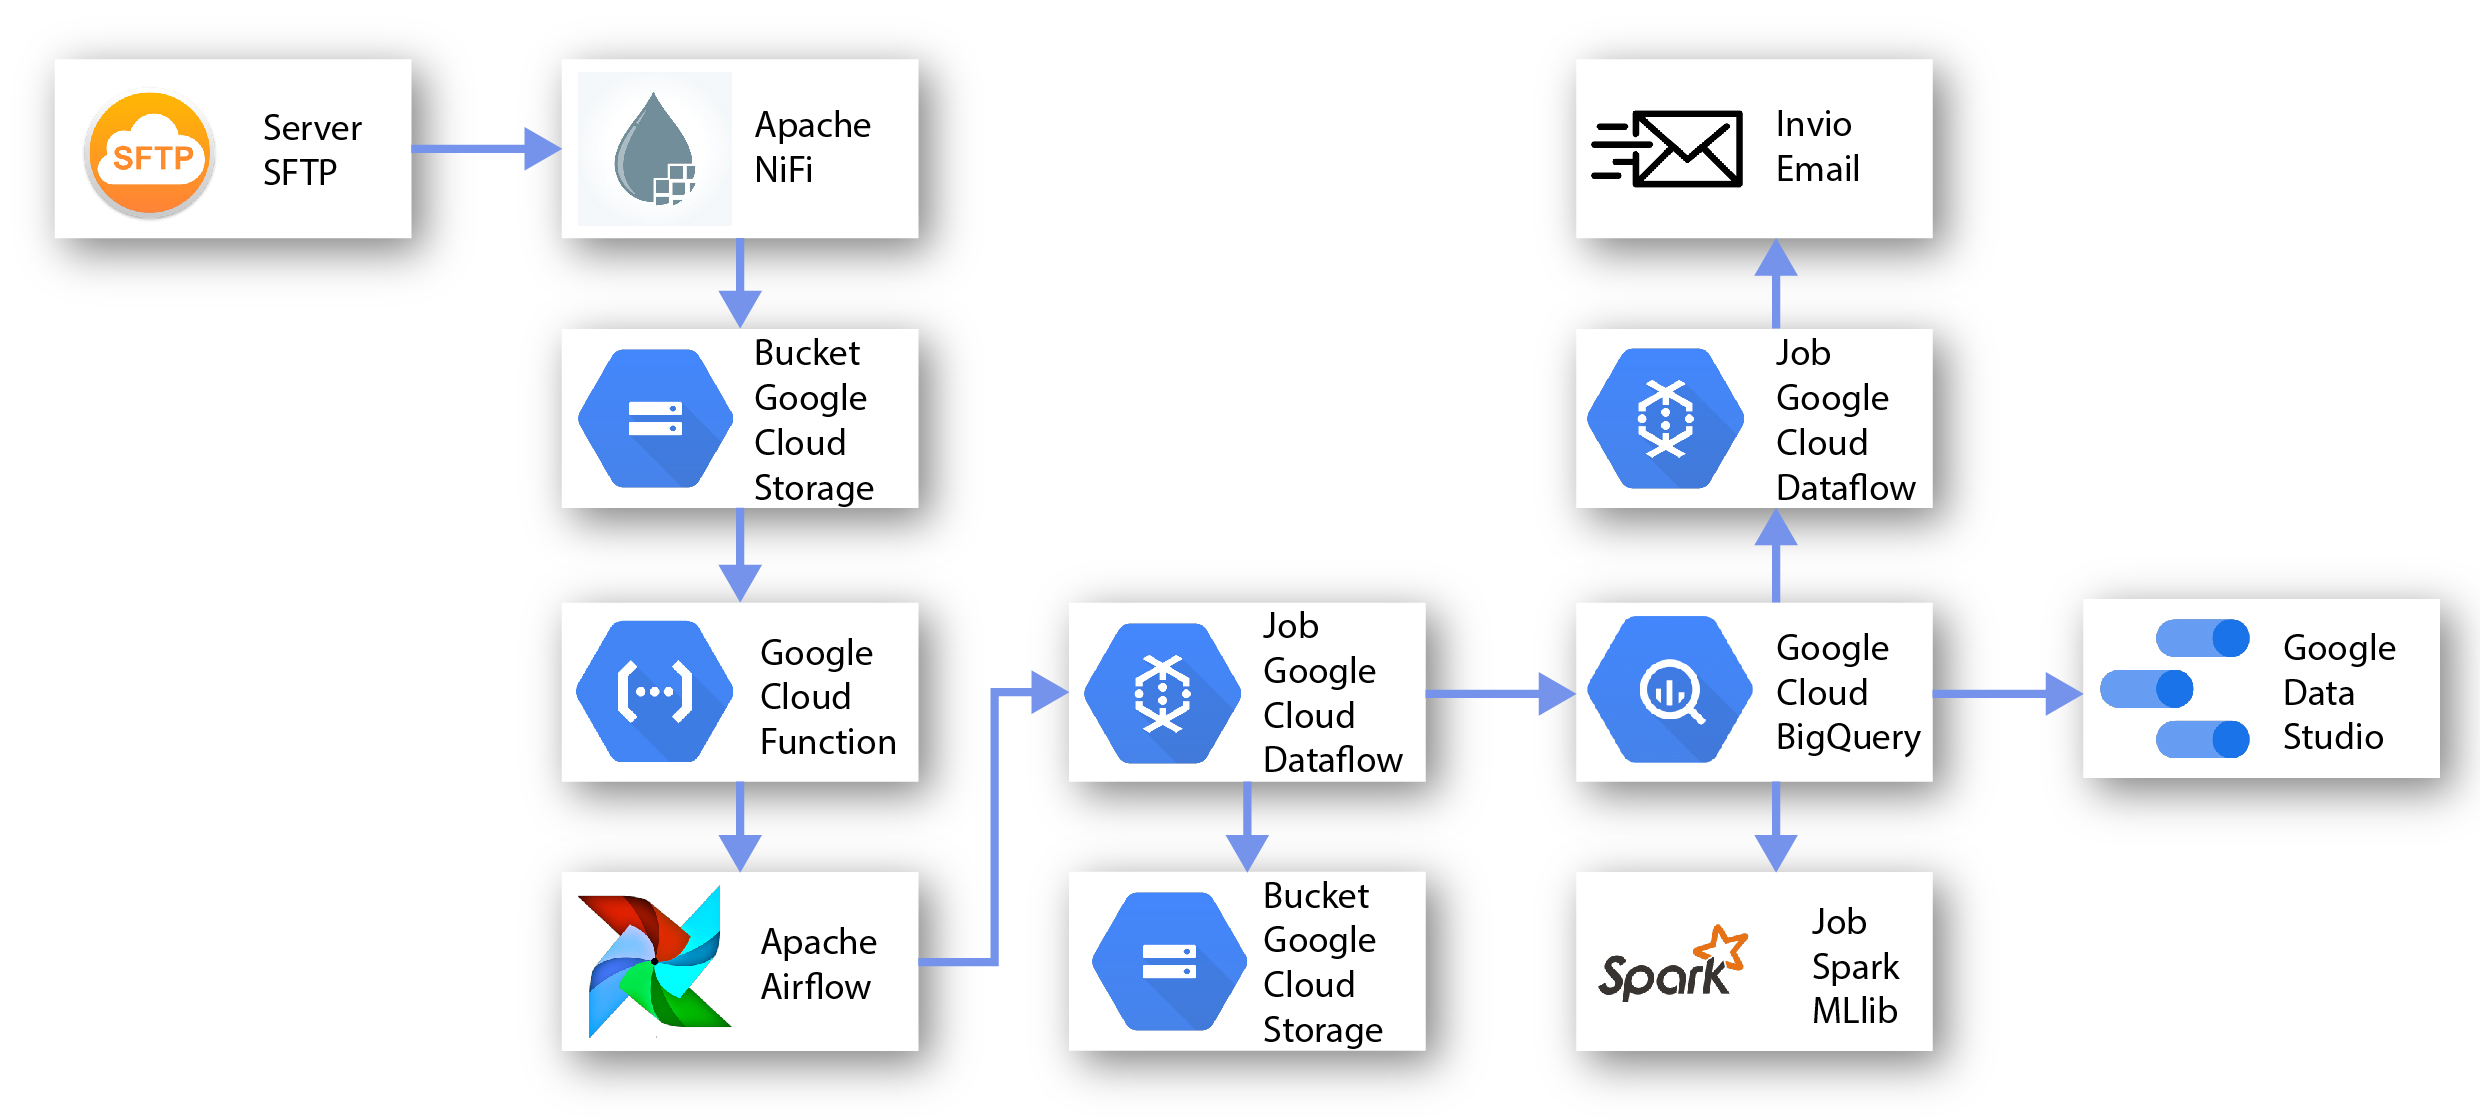
\includegraphics[scale=0.65]{figures/Schema_complessivo_ridotto}
	\caption[Workflow progetto	.]{\emph{Workflow} progetto.
		\label{fig:workflow}}
\end{figure}	
L'integrazione delle tecnologie elencate in §\ref{GoogleCloud}{}, ha portato a stabilire un vero e proprio ciclo di vita del dato.
La gestione del dato inizia con il caricamento dei file all'interno di un server SFTP da parte del cliente. Tramite Apache NiFi, avviene una prima pre-elaborazione. Vengono accettati solo file con estensione \emph{XML} o \emph{evtx}, nel caso di file differenti questi vengono scartati. La pre-elaborazione consiste nella validazione e conversione dei file \emph{evtx} in \emph{XML} così da uniformare e generalizzare il più possibile le procedure di \emph{ingestion} dei dati.
\\
Attraverso Apache Nifi, i file vengono spostati all'interno di Google Cloud Storage, il quale, al trasferimento di ogni file, provoca l'avvio delle Google Cloud Function. Come descritto all'interno di §\ref{GoogleCloudFunction}{}, Google Cloud Function offre la possibilità di essere avviata tramite eventi, in questo caso troviamo l'utilizzo dell'origine Cloud Storage di tipo \emph{finalize}. Attraverso le Function, viene avviato il processo di \emph{ingestion} sul file appena trasferito tramite l'attivazione del file DAGs all'interno di AirFlow.
\\
La fase di \emph{Data Processing} è composta da alcuni \emph{job} Google Cloud Dataflow scritti in Python e caratterizzati dall'utilizzo di Apache Beam per la creazione delle pipeline dei dati.
Il processamento dei dati è mirato al rendere i dati maggiormente leggibili e consultabili decodificandoli e aggregandoli. Dopodiché, gli stessi vengono scritti all'interno di apposite tabelle Google Cloud BigQuery.
\\
Per quanto riguarda la \emph{Data Analysis}, il cliente ha richiesto due tipologie distinte di analisi dei dati.
La prima riguardava il confronto dei dati giornalieri con i dati storicizzati, per capire se fossero state riscontrate possibili anomalie (come ad esempio la forte diminuzione dell'utilizzo di determinati strumenti), e nel caso di esito positivo, immediatamente notificarlo al responsabile del settore tramite email.
La seconda riguardava la classificazione degli utenti che utilizzano il sistema del cliente per trovare eventuali cambi di categorie non autorizzate (che corrispondono ad anomalie). Per concludere il processo da dato ad informazione, abbiamo costruito un sistema che, tramite Kafka e secondo lo schema produttore-consumatore in \emph{streaming}, invia dei dati ad un algoritmo di \emph{machine learning} sviluppato tramite Apache Spark (più in particolare tramite la libreria Apache Spark MLlib) che raggruppa gli utenti su base settimanale, conserva i valori dei raggruppamenti e verifica che ogni utente non abbia cambi di cluster in modo anomalo.\\
Al termine di questo processo, abbiamo il definitivo passaggio da semplice dato ad effettiva informazione per cliente tramite i report e le \emph{dashboard} riassuntive di Google Data Studio. Questa fase viene di norma chiamata \emph{Data Integration}.
\begin{figure}[h!]
	\centering
	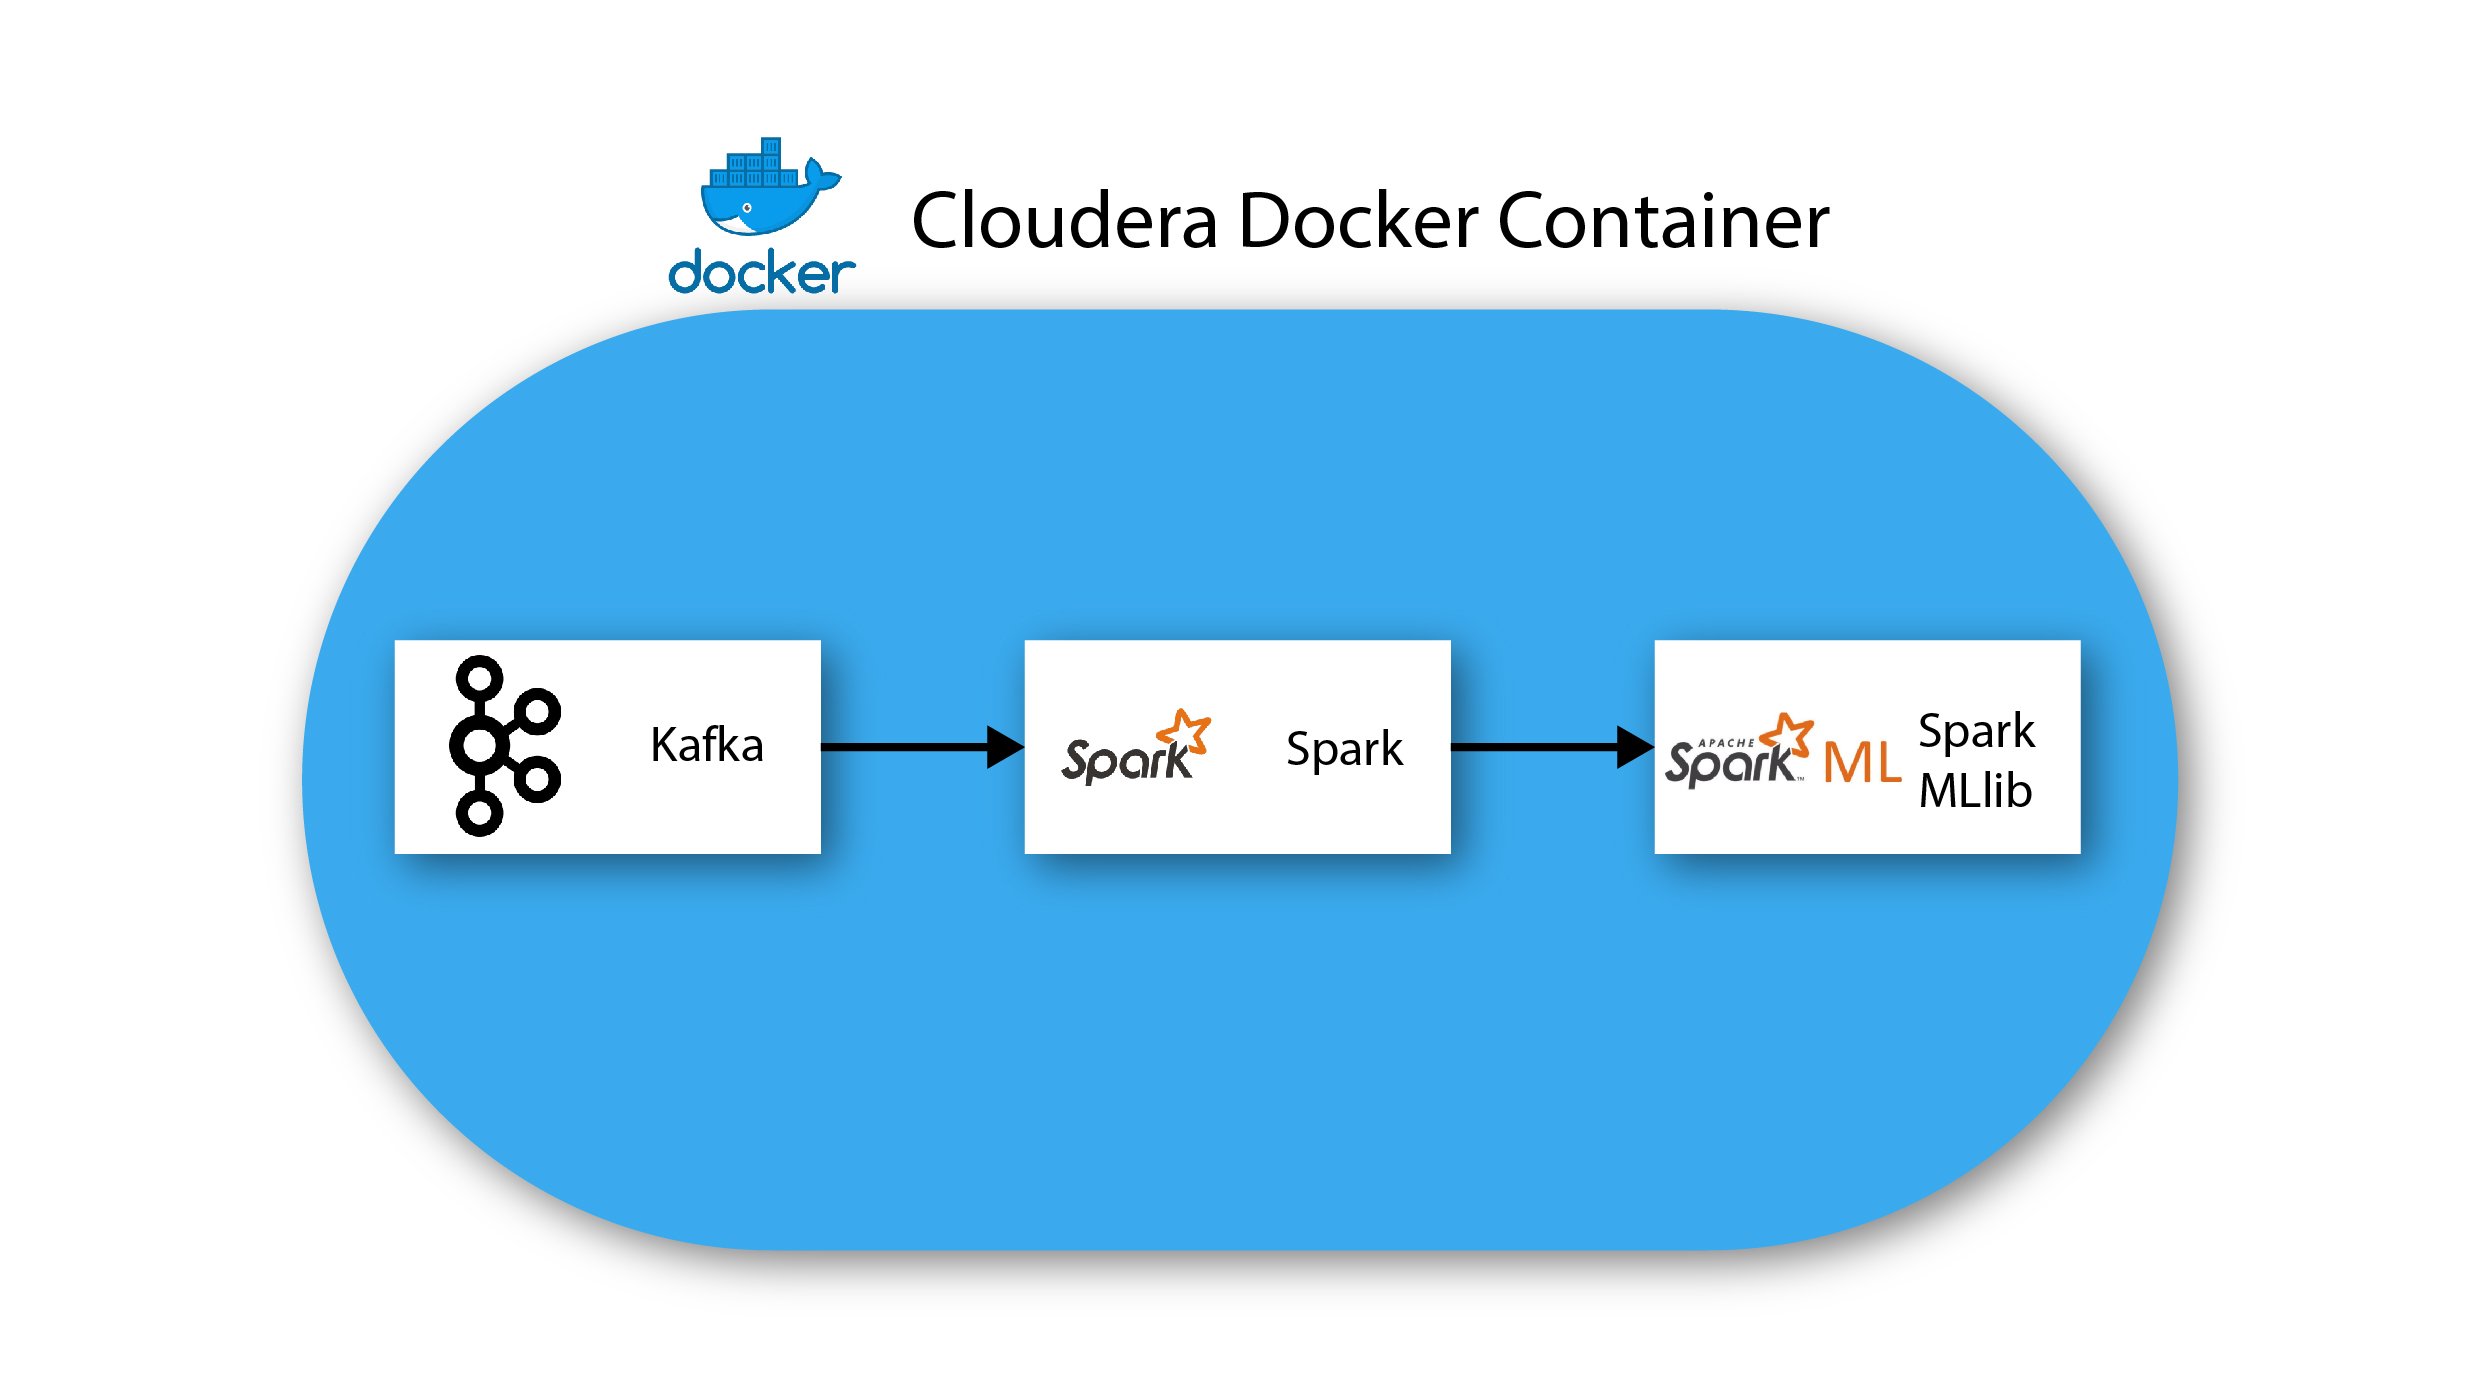
\includegraphics[scale=0.5]{figures/kafka_spark}
	\caption[Workflow integrazione Kafka e Spark.]{\emph{Workflow} integrazione Kafka e Spark all'interno di Docker Container.
		\label{fig:workflow2}}
\end{figure}	
\subsection{Valutazione Data Analysis}
La valutazione della fase di Data Analysis è stata svolta in modi diversi per le due tipologie richieste dal cliente.
\\
La valutazione del confronto dei dati giornalieri con quelli storicizzati è stata fatta attraverso la creazione di dati simulati, inserendo anomalie di diversa entità così da calibrare al meglio la soglia di invio delle email al responsabile aziendale. Il \emph{dataset} creato era composto da 7500 elementi, di cui 13 erano anomalie.
\\
Seguendo l'esempio portato in precedenza, nel caso in cui l'utilizzo di un dato strumento fosse aumentato vertiginosamente il responsabile sarebbe stato avvisato. La soglia minima per attestare un'anomalia, in accordo con il cliente, è stata fissata al 50\% in più della media dei dati storicizzati. All'interno dell'email al responsabile, troviamo anche l'indicazione di quanto la soglia sia stata superata, in modo da tenere traccia e migliorare la resa delle segnalazioni.
\\
Al termine della fase di test, i risultati ottenuti sono stati valutati come accettabili, con un 90\% circa di \emph{precision} e 85\% circa di \emph{recall}.
\\
Per quanto riguarda la valutazione dell'algoritmo di \emph{clustering}, anche qui troviamo la creazione di dati simulati con all'interno utenti appositamente anomali, in questo caso il dataset comprendeva 12000 record di cui 21 anomali. Ho notato che l'algoritmo utilizzato non è ottimale, infatti con l'utilizzo degli stessi dati potrebbe tendere alla scelta di diversi nuclei dei \emph{cluster} a seconda dei punti iniziali dell'algoritmo. Per questo motivo la valutazione è soddisfacente, ma migliorabile tramite l'utilizzo di algoritmi di \emph{clustering} più precisi ed efficienti. Nella fase di test i risultati non sono stati ottimali: 75\% circa di \emph{precision} e 60\% circa di \emph{recall}. Per questo motivo vi sarà bisogno di una fase di studio del problema aggiuntiva.

\section{Tecnologie}
\subsection{Google Cloud}\label{GoogleCloud}
Il principale servizio utilizzato durante il progetto è stato Google Cloud, in esso troviamo una moltitudine di strumenti utili allo sviluppo, all'esecuzione e all'interazione di progetti riguardanti \emph{big data} e Intelligenza Artificiale. Inoltre, importante risulta la possibilità di consultare, manipolare e presentare i dati.
Il progetto Google Cloud (anche detto Google Cloud Platform o GCP), viene lanciato nel 2008 con uno dei suoi servizi di punta ancora oggi  \Gls{App Engine}. Nell'arco degli anni sia il bacino di utenti, sia i servizi offerti sono via via aumentati. Oggigiorno i suoi clienti \cite{clienti} sono molti, tra cui grandi aziende, e le funzionalità di spicco sono molteplici, i campi di maggiore interesse riguardano strumenti di Computazione, Immagazzinamento \& \emph{Database}, \emph{big data}, \emph{Cloud AI} e \emph{IoT}.
\\
Per quanto riguarda l'esperienza personale, ho trovato Google Cloud un buon servizio, con dei problemi da risolvere sulla completezza della documentazioni e a volte con grafiche da migliorare, ma comunque un ottimo compromesso tra qualità e prezzo.
\\
Il resto della sezione introduce il prodotti e i servizi GCP utilizzati durante lo stage.
\begin{figure}[h!]
	\centering
	
\includegraphics[scale=0.3]{figures/google-cloud-platform}
	\caption[Logo Google Cloud Platform.]{Logo Google Cloud Platform.
		\label{fig:logoGCP}}
\end{figure}	
\subsubsection{Google Cloud Storage}
Lanciato nel 2010, Google Cloud Storage è il servizio di hosting dei file della piattaforma. All'interno ogni utente può scegliere in che modalità salvare i dati (zona del mondo, carico di lavoro e frequenza d'accesso), così da trovare la soluzione maggiormente adatta ai propri bisogni.
I suoi punti di forza sono:
\begin{itemize}
	\item Interoperabilità: possibilità di interfacciarsi con strumenti e servizi di aziende terze (come Amazon S3);
	\item Consistenza: tutte le operazioni sono svolte secondo il principio di \Gls{atomicità};
	\item Controllo di accesso: possibilità di definire l'accesso ad un singolo oggetto o \emph{\gls{bucket}} a seconda della categoria di appartenenza degli utenti;
	\item \emph{Resumable Upload}: in caso di fallimento di un \emph{upload}, questo può essere continuato/ricominciato.
\end{itemize}

Per quanto riguarda l'esperienza d'utilizzo, si è rivelato un ottimo servizio di \emph{storage}, l'abilitazione di un'unica API rende disponibile l'intero pacchetto di funzionalità e ciò l'ho trovato molto comodo.
\subsubsection{Google Cloud BigQuery}
Servizio lanciato insieme a Google Cloud Storage nel 2010, Google Cloud BigQuery , è lo strumento che permette di interagire e analizzare grandi moli da dati, definito come un \emph{\gls{data warehouse}}. All'interno di GCP, vi è un'apposita interfaccia utente per utilizzarlo. Si basa su tabelle codificate in formato \emph{JSON} e sulla quale vengono processate query in standard SQL \cite{standardSQL} tramite avanzati algoritmi di \Gls{MapReduce}.
\\I principali punti di forza sono:
\begin{itemize}
	\item La piattaforma rende disponibile la creazione e distruzione di tabelle basati su schemi JSON, inoltre rende disponibile l'import e l'export di dati in formati come \emph{CSV} e J\emph{SON};
	\item La semplicità del linguaggio SQL con scalabilità e prestazioni che solo i servizi cloud riescono a dare;
	\item Un'ottima integrazione con servizi e \emph{API} esterni, per la raccolta e l'utilizzo dei dati;
	\item Possibilità di garantire l'accesso ad uno o più categorie di utenti;
	\item Possibilità di interagire con strumenti di \emph{machine learning} nativi di Google e non (come TensorFlow).
\end{itemize}

L'opinione del team di sviluppo riguardo lo strumento è molto positiva sopratutto grazie alla scalabilità automatica che rende semplice e veloce l'utilizzo delle query su grandi moli di dati, un possibile punto di debolezza può essere trovato nell'utilizzo in sola lettura dei dati esistenti, quindi non vi è la possibilità di modifica dei record se non un nuovo inserimento.
\subsubsection{Google Cloud Dataflow}
Rilasciato al pubblico nel 2015, Google Cloud Dataflow è lo strumento che permette di processare pipeline per l'integrazione, la preparazione e l'analisi di grandi quantità di dati.
Il modello di pipeline consigliato è quello di Apache Beam che vedremo in seguito.
\\ Tra i maggiori punti di forza troviamo:
\begin{itemize}
	\item Creazione di pipeline secondo modelli già esistenti o personalizzati dall'utente;
	\item Composizione di pipeline, e quindi \emph{job} specifici, direttamente da codice;
	\item Possibilità di utilizzo di dati da molteplici fonti, non solo da strumenti Google;
	\item Ottima scalabilità interna in base agli effettivi bisogni del lavoro in esecuzione;
	\item Buona granularità della specificazione dei parametri di esecuzione\cite{parametridiesecuzione} della pipeline;
	\item Visualizzazione grafica della pipeline. 
\end{itemize}

\begin{figure}[h!]
	\centering
	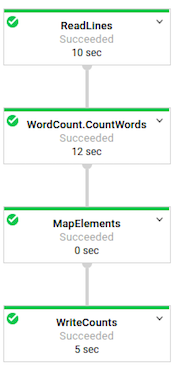
\includegraphics[scale=1]{figures/dataflow-job-full}
	\caption[Esempio di pipeline dataflow.]{Esempio di pipeline Dataflow
		\label{fig:pipelinedataflow}}
\end{figure}	


Per quanto concerne l'utilizzo di questo prodotto, il team si esprime con un giudizio più che positivo dato anche la grande quantità di documentazione disponibile.
\subsubsection{Google Cloud Function}\label{GoogleCloudFunction}
Rilasciato in beta nel 2017, Google Cloud Functions è il perfetto intermediario tra gli eventi che vengono scaturiti nel cloud e l'invocazione di API. Le origini degli eventi supportati sono:
\begin{itemize}
	\item Cloud Pub/Sub;
	\item Cloud Storage;
	\item HTTP;
	\item Stackdriver Logging;
	\item Firebase. 
\end{itemize}
Inoltre, per ogni tipologia di evento vi sono ulteriori specificazioni che non verranno trattate tutte in modo estensivo in questo elaborato.
\\
Per quanto concerne l'utilizzo svolto durante il progetto, il team ritiene questo strumento valido e con ottime potenzialità e margini di miglioramento. Uno svantaggio molto importante da sottolineare è la scarsa documentazioni presente nelle fonti ufficiali.
\subsection{Apache NiFi}
\begin{quotation}
An easy to use, powerful, and reliable system to process and distribute data.
	\qauthor{NiFi Creator}
\end{quotation}
La descrizione che viene data nella documentazione di NiFi \cite{NiFi} riassume alla perfezione le caratteristiche di questo strumento e ciò che ci permette di fare.
\\
Innanzitutto, le sue funzioni sono proprio quelle di automatizzare lo "scorrere" del flusso dati all'interno del sistema in cui viene utilizzato. Le funzionalità sono molteplici e ben rodate, vanno dal semplice spostamento dei file, al filtraggio, composizione e conversione in diversi formati. La documentazione è molto esauriente, spiegando anche più del necessario tutti i passaggi da seguire per utilizzare un determinato componente. La semplicità e l'intuitività nel costruire il flusso di dati, rendono l'esperienza utente decisamente piacevole, anche grazie all'interfaccia grafica semplice e intuitiva. Altro punto a favore è l'affidabilità del prodotto e la grande quantità di componenti disponibili orientati alla sicurezza, così da rendere il passaggio di informazioni il più sicuro possibile.
\begin{figure}[h!]
	\centering
	\includegraphics[scale=0.1]{figures/apache-nifi-logo}
	\caption[Logo Apache NiFi.]{Logo Apache NiFi
		\label{fig:LogoApacheNiFi}}
\end{figure}
\subsubsection{Google Data Studio}
Lanciato nel 2016, Google Data Studio è lo strumento di creazione e visualizzazione dei dati attraverso report e \emph{dashboard}. L'idea che sta alla base di questo \emph{tool} è la condivisione dei dati che sono presenti all'interno di GCP attraverso tabelle e grafici.
\\ I maggiori vantaggi nell'utilizzarlo sono:
\begin{itemize}
	\item Accesso ai dati personali di GCP;
	\item Possibilità di integrare i dati fra di loro con query standard SQL;
	\item Condivisione a gruppi di utenti. 
\end{itemize}

Durante l'esperienza lo strumento si è rivelato molto acerbo nelle sue funzionalità e nell'utilizzo, oltre a dover attendere troppo tempo per il caricamento di dati e grafici. L'idea alla base è ottima, dato che vi è la possibilità di utilizzare i dati all'interno di GCP anche in continuo aggiornamento, d'altro canto la documentazione e l'interfaccia utente non rendono semplice quanto potrebbero la creazione di un report aziendale da presentare al cliente.	
\subsection{Apache Beam}
Apache Beam è un implementazione del modello Dataflow \cite{modelloDataflow}, esso infatti fissa come definire ed eseguire pipeline sui dati di tipo \emph{ETL} (\emph{extract}, \emph{transform}, and \emph{load}), \emph{batch} e \emph{streaming} continui. Questo progetto nasce dopo il rilascio di un \gls{SDK} contenente un implementazione del modello Dataflow da parte di Google nel 2014, nel 2016 Google decise di concedere il core del proprio SDK per costituire il progetto \Gls{OpenSource} Apache Beam.
\\ I concetti alla base di questa implementazione, e quindi del modello Dataflow, possono essere riassunti nel cercare un modello il quale riesca a definire ed eseguire pipeline di tipo \emph{batch} e \emph{streaming} allo stesso tempo, senza dover differenziare le pipeline come nel modello \emph{Lambda architecture} \cite{Lambdaarchitecture}.
\\ Un tipico utilizzo di una pipeline può essere il seguente:
\begin{figure}[h!]
	\centering
	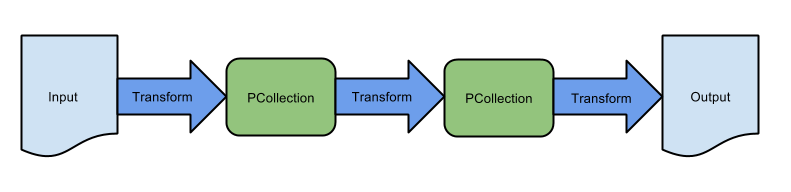
\includegraphics[scale=0.5]{figures/design-your-pipeline-linear}
	\caption[Esempio utilizzo Apache Beam. ]{Esempio utilizzo Apache Beam.
		\label{fig:beam}}
\end{figure}	
\begin{itemize}
	\item Creazione della \emph{Pipeline};
	\item Creazione di una \emph{PCollection} da dei dati di input;
	\item Applicazione di \emph{PTrasforms} sulla \emph{PCollection};
	\item Scrittura dei dati all'interno di un file.
\end{itemize}
Le azioni di maggiore interesse stanno nelle PTrasforms, infatti rende possibile processare ogni singolo elemento delle PCollection, effettuare raggruppamenti per uno o più elementi, unire  e partizionare le \emph{PCollection}.
La documentazione a disposizione è decisamente idonea e precisa rispetto alla potenzialità di utilizzo. Inoltre, essendo un progetto OpenSource vi è la possibilità di collaborare al continuo sviluppo, e quindi al successo, che questa tecnologia sta avendo.
\subsection{Apache AirFlow}
Apache AirFlow è una piattaforma per creare, schedulare e monitorare \gls{workflows}. Airflow, inoltre, cerca la soluzione più performante per l'esecuzione dei task, creando un Grafo Aciclico Diretto (meglio conosciuto come "\gls{DAGs}" cioè "Directed Acyclic Graphs") in modo da riconoscere le dipendenze tra i compiti stessi ed eseguire i task con meno dipendenze.
La scelta di utilizzare questa tecnologia è stata presa sia per la già precedente esperienza aziendale con essa, sia perché completamente compatibile e già installata all'interno di Google Cloud Composer. Data la sua notevole compatibilità ci ha permesso di soddisfare un requisito del cliente riguardante l'\emph{ingestion} in tempo reale dei dati inviati.
\subsection{Docker}
Nato nel 2013, Docker è una piattaforma software che permette di creare \emph{build}, testare e distribuire applicazioni con la massima rapidità. Docker raccoglie il software in unità standardizzate chiamate container che offrono tutto il necessario per la loro corretta esecuzione. L'utilizzo di Docker in questo progetto per la parte del sistema di classificazione è coerente con i principali pregi e funzionalità offerte da questo strumento.
Tra le principali funzionalità troviamo:
\begin{itemize}
	\item Integrazione con le maggiori infrastrutture;
	\item Portabilità;
	\item Controllo di versione e riutilizzo dei componenti;
	\item Facilità nella condivisione.
\end{itemize}
\subsection{Kafka}
Apache Kafka è una piattaforma \emph{open source} di \emph{stream processing}, mira a creare una piattaforma a bassa latenza ed alta velocità per la gestione di dati in tempo reale.
Apache Kafka è quindi un broker di messaggistica, dato che una volta definiti dei \emph{topic}, la domanda di dati del \emph{consumer} e l'offerta di dati del \emph{producer} è mediata da un Kafka server. Questo offre alcuni vantaggi:
\begin{itemize}
	\item Memorizzazione dei messaggi in modo da prevenire la perdita dei dati;
	\item Alta flessibilità di variazione nel flusso, quindi controllo e prevenzione di eventuali colli di bottiglia;
	\item Tollerante agli errori;
	\item Buona scalabilità.
\end{itemize}
Nel progetto, funge da intermediario tra il database e il sistema di classificazione, per mantenere un flusso continuo di dati e scovare eventuali operazione sospette.
\subsection{Apache Spark}
Sviluppato all'interno dell'Università della California e poi donato ad Apache, Spark è un \emph{framework} per il calcolo distribuito. 
All'interno di Apache Spark vi troviamo una moltitudine di funzionalità e librerie, tra cui Apache Spark MlLib.
\subsubsection{Apache Spark MlLib}
All'interno di questa libreria, troviamo alcuni tra i più famosi e preformanti algoritmi di \emph{machine learning}. Questa libreria è stata utilizzata per la sua semplicità di utilizzo e per le sue prestazioni ottime nei confronti delle altre librerie.
\\
\textbf{K-Means} \cite{k-means} è  l'algoritmo utilizzato nel progetto, scelto per iniziare una fase di perlustrazione della libreria e mantenuto dato lo stato ancora non avanzato del progetto nella parte di analisi ed utilizzo delle informazioni.
\section{Strumenti}
Gli strumenti di lavoro utilizzati sono stati scelti in base agli standard aziendali e per mantenere la massima compatibilità con il pacchetto GCP.
\\
Python è stato il linguaggio di riferimento per il progetto. La decisione è stata presa tenendo in considerazione i linguaggi supportati da GCP e pensando all'utilizzo nella parte di riconoscimento delle anomalie. Infatti, la numerosa presenza di librerie di supporto e la presenza di molta documentazione a supporto per il medesimo linguaggio ha spostato l'ago della bilancia su Python al posto di linguaggi comunque molto diffusi e conosciuti come Java. Inoltre, essendo un linguaggio non studiato durante i corsi di laurea, ho ritenuto fosse un'ottima occasione per iniziare ad utilizzarlo.
\\
PyCharm è stata conseguenza diretta dell'uso di Python, dato che è un'ottimo \emph{IDE} il quale offre assistenza durante la codifica. Oltre a garantire una buona compatibilità con GCP, fondamentale per il ruolo che ricopre.
\\
Aderendo alle consuetudini aziendali, il sistema di controllo di versione adottato è Git, attraverso la piattaforma GitLab. Si è inoltre deciso di utilizzare GitLab Mattermost per la comunicazione all'interno del team.

\begin{figure}[h!]
	\centering
	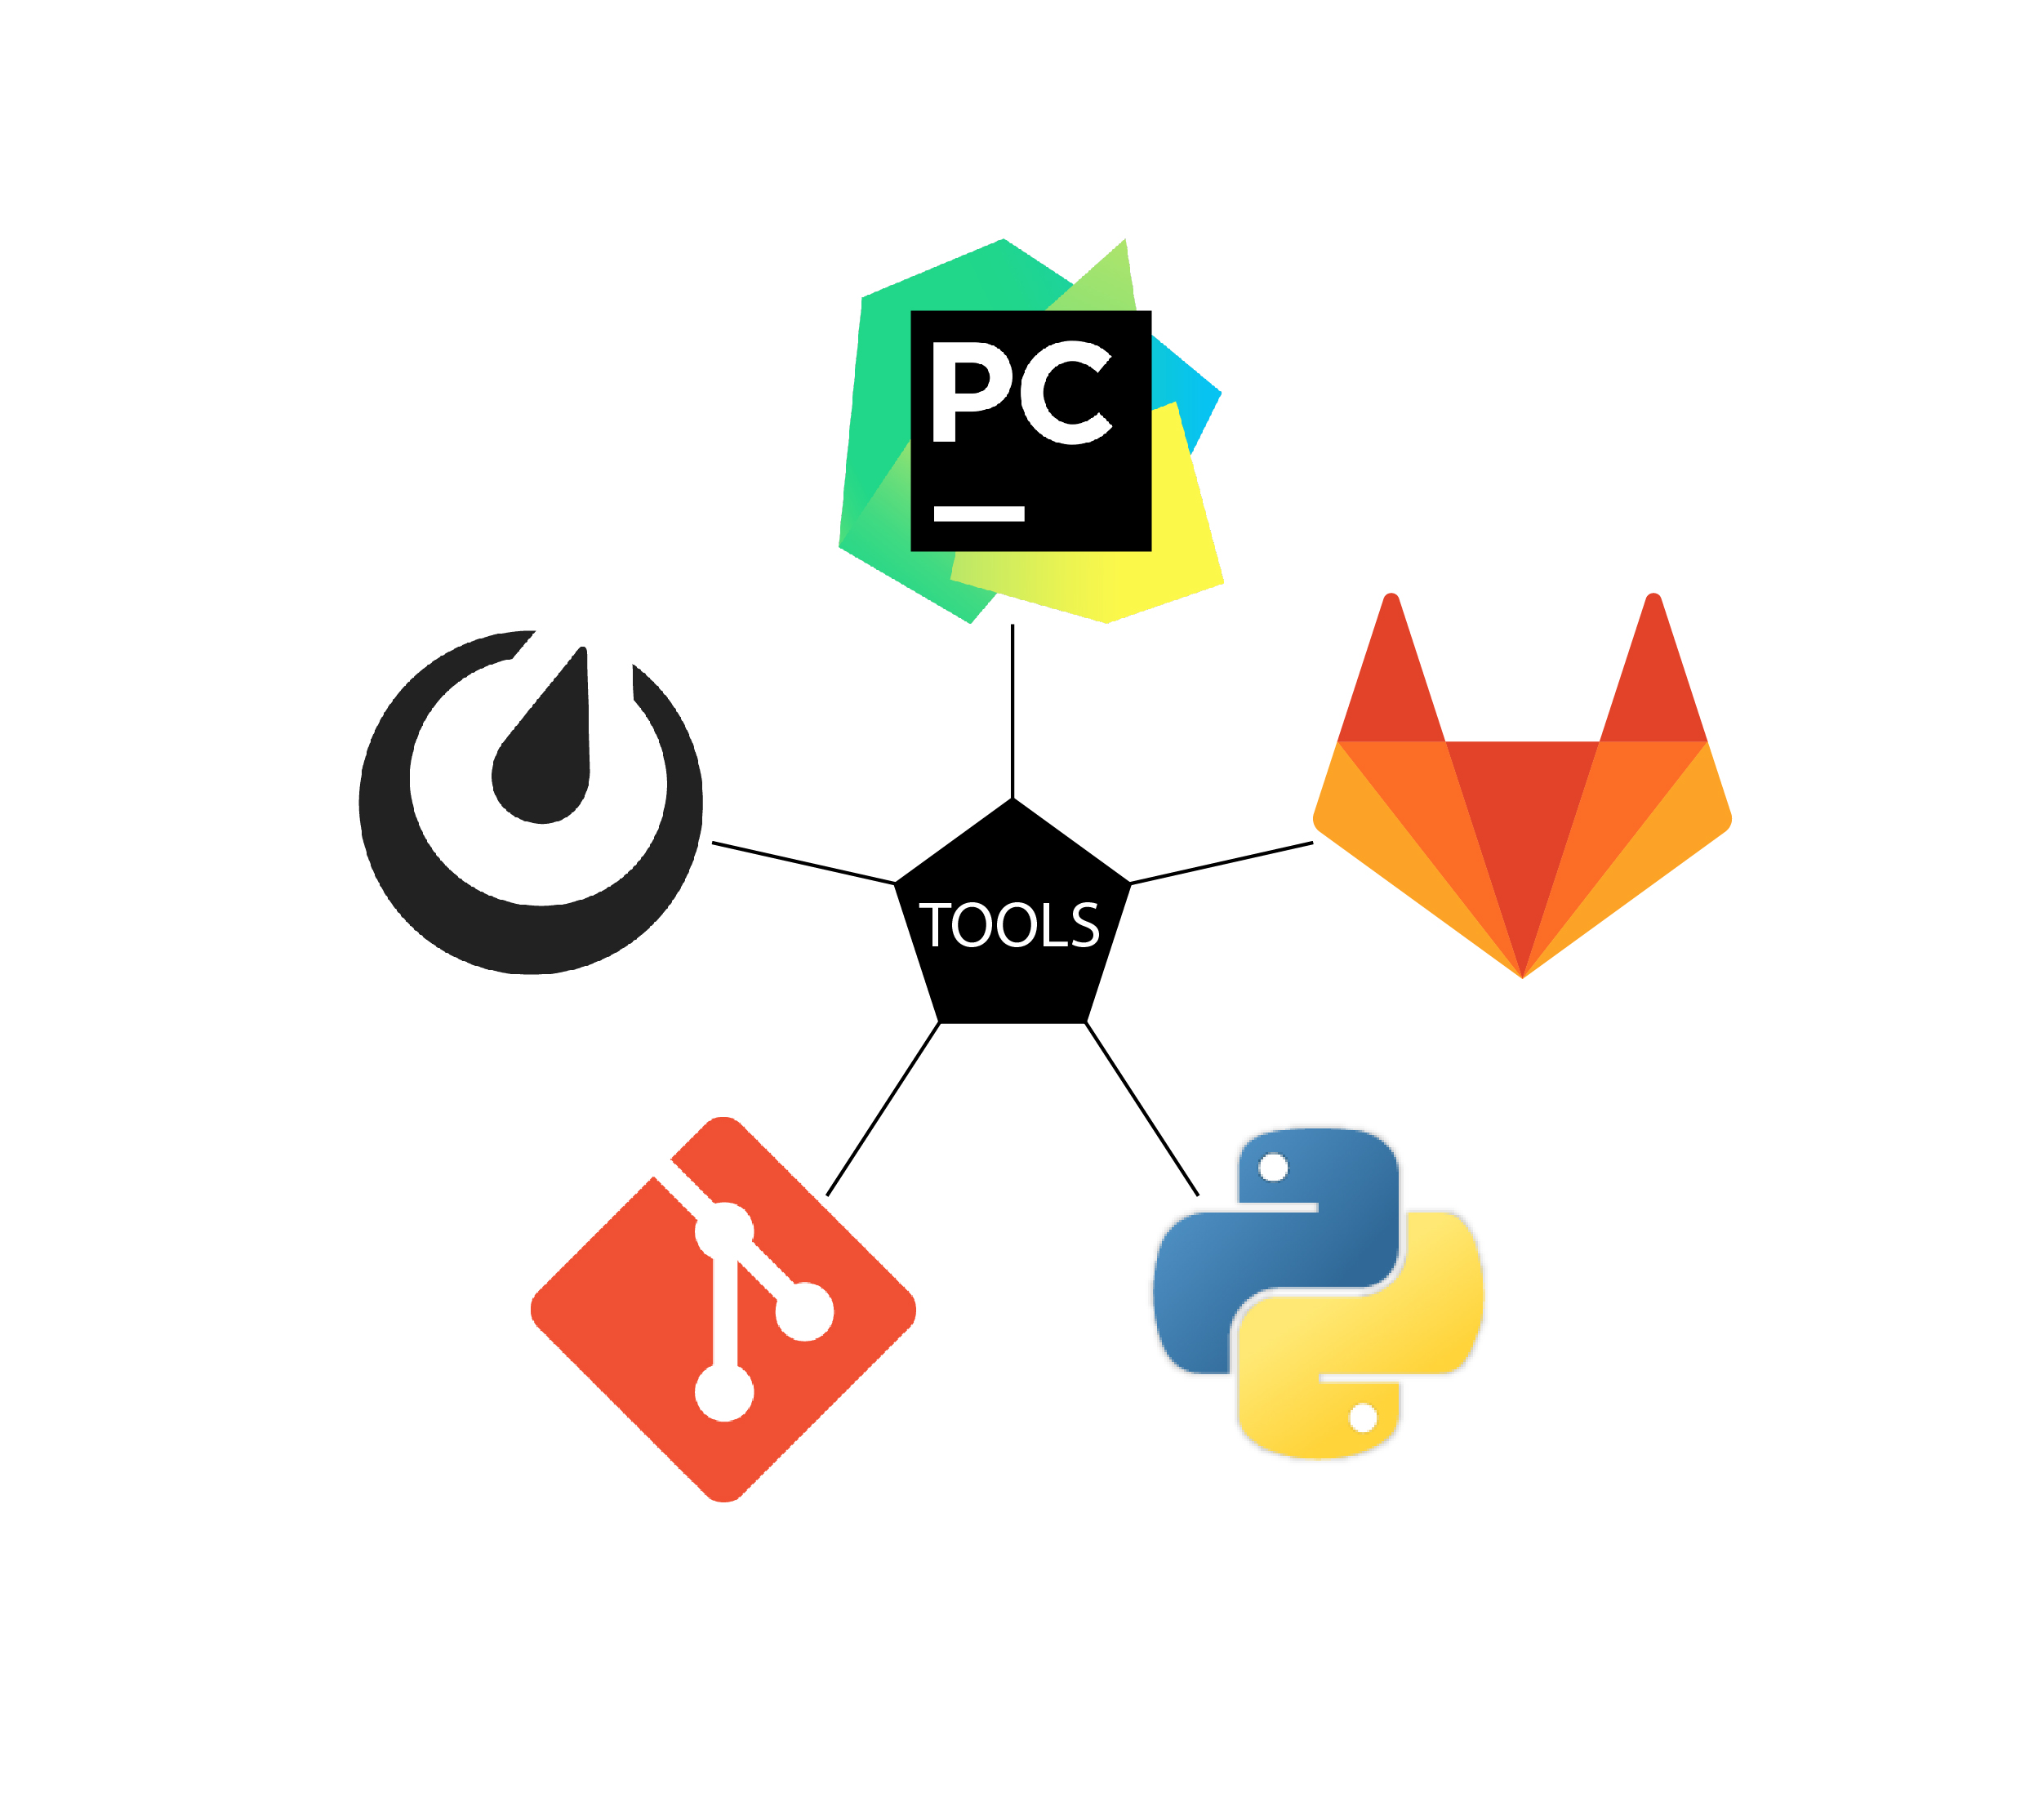
\includegraphics[scale=0.4]{figures/pentagono_grande-03}
	\caption[Loghi strumenti utilizzati.]{Loghi strumenti utilizzati.
		\label{fig:loghi}}
\end{figure}	